
\chapter{Marco Teórico} \label{chap:marcoteorico} 
Dentro de este capítulo se realizó una investigación tipo exploratoria, ya que se pretende dar una visión general acerca de las nuevas técnicas agrícolas de interiores como lo es la hidroponía. Este tipo de investigación se realiza especialmente explorando los conceptos y aplicaciones de tecnologías dentro de un sistema hidropónico de tipo DFT y su reconocimiento en el área agrícola. Dentro de estas técnicas suelen surgir nuevos fenómenos, que precisamente por su alta novedad, se admiten distintos tipos de estructuras de acuerdo con las necesidades de cada uno de los agricultores, en cuanto a su disposición de recursos y así generar un sistema capaz de realizar un control automático.

\section{Hidroponía}
\subsection{Técnicas de hidroponía}
La palabra hidroponía proviene de las palabras griegas HYDRO (agua) y PONOS (trabajo o mano de obra), que literalmente significa trabajo en el agua. Es un conjunto de técnicas que hacen posible el cultivo de plantas en un entorno libre suelo o algún sustrato. La hidroponía permite estructuras simples o complejas produzcan plantas herbáceas en lugares como techos, suelos pobres, terrenos irregulares, invernaderos con o sin calefacción. Con base en este concepto, se están desarrollando nuevas técnicas donde se aporta una solución nutritiva estática o circulante al sistema, considerando las necesidades de las plantas como su temperatura, humedad, agua y nutrientes. Los requerimientos de nutrientes adecuados son suministrados usando agua y una solución nutritiva para cultivar plantas que puedan crecer \cite{beltrano_gimenez}.

Dentro de la hidroponía hay distintos tipos de sistemas hidropónicos \cite{dholwani2018introduction}, donde pueden clasificarse de dos formas:
\begin{itemize}
\item \textbf{Método circulante (closed system).} Las plantas cultivadas se encuentran en una solución nutritiva donde sus raíces se mantienen suspendidas directamente en una solución nutritiva. Estos cultivos también pueden llamarse de flujo continuo. Existen estos tipos de sistemas hidropónicos circulantes:
\newpage
\begin{itemize}
\item \textbf{Sistema hidropónico basado en la técnica de película de nutrientes (NFT, por sus siglas en inglés).} El sistema NFT es uno de los más populares entre los cultivadores hidropónicos domésticos. Principalmente debido a su diseño simple. Estos sistemas también son los más adecuados y utilizados para el cultivo de plantas más pequeñas de crecimiento rápido, como los diferentes tipos de lechuga.

\item \textbf{Sistema hidropónico DFT.} Estos sistemas son uno de los tipos de sistemas hidropónicos más utilizados en todo el mundo, tanto para cultivadores domésticos como comerciales, pues su disposición puede ser muy variada. Este tipo de sistema se basa en un método de cultivo en el que las raíces de las plantas se colocan en una capa de agua profunda en una solución nutritiva. Los sistemas DFT se encuentran entre los sistemas más utilizados en el mundo debido a su estructura sin restricciones. La función principal de este sistema es hacer circular la solución nutritiva, mientras las raíces de las plantas están en agua las 24 horas del día. Dado que el sistema es cerrado, la técnica se clasifica como un método circulante. Una representación gráfica de este sistema se muestra en la figura \ref{dft1}.
\end{itemize}

\item \textbf{Método no circulante (open system)}.
\begin{itemize}
\item \textbf{Sistema hidropónico raíz flotante.} En este método, las plantas se encuentran en una lámina o balsa, generalmente de unicel, que flota sobre la solución nutritiva de modo que sus raíces están sumergidas dentro de la solución. Una bomba de aire proporciona a las raíces el oxígeno necesario para su óptimo desarrollo. 
\item \textbf{Aeroponía:} Es una técnica en la que las raíces se encuentran suspendidas en el aire, dentro de un medio oscuro, y se nebulizan con solución nutritiva cada pocos minutos.
\end{itemize}
\end{itemize}

\begin{figure}[!ht]
\centering
         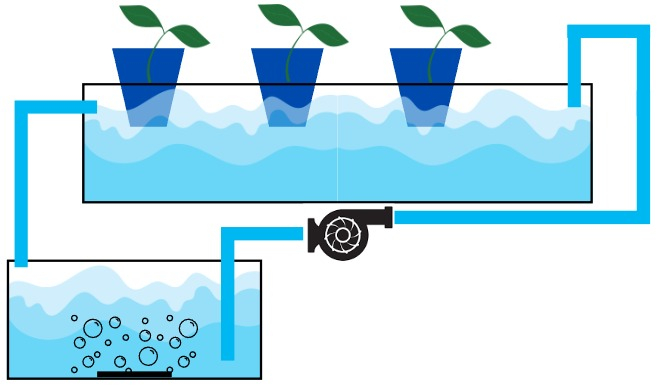
\includegraphics[scale=0.45]{imgs/dft.jpeg} \\
     \caption{Diseño básico de un sistema DFT.}\label{dft1}
\end{figure}

\subsection{Solución nutritiva}
El éxito en la producción de una gran diversidad de cultivos hidropónicos dependerá mucho de la nutrición mineral de las plantas. Para sistemas hidropónicos o semi hidropónicos, la solución nutritiva se usa para nutrir inorgánicamente a las plantas, con el fin de aportar los elementos nutritivos para que las plantas se desarrollen correctamente, tanto en macronutrientes (nitrógeno, fósforo, potasio, calcio, magnesio y azufre) como en micronutrientes (hierro, manganeso, boro, zinc, cobre, molibdeno, cloro) \cite{favela_2006}.
\begin{itemize}
\item \textbf{Macronutrientes.} También conocidos como nutrientes primarios, incluyen elementos como nitrógeno (N), fósforo (P) y potasio (K), Los nutrientes primarios del suelo son fáciles de agotar porque las plantas consumen enormes cantidades de estos nutrientes para crecer \cite{Meselmani22}.
\item \textbf{Micronutrientes.} También llamados nutrientes secundarios, son nutrientes que se pueden regeneran en los cultivos de suelo. Para los cultivos hidropónicos, el número de partes de micronutrientes necesarios se pueden calcular con base en el tipo de cultivo y darles suficiente para crecer más grande, mejor y más rápido. Los micronutrientes también se conocen como elementos traza \cite{Meselmani22}.
\end{itemize}

En este proyecto se emplearon 5 grupos de nutrientes en forma de sales, con base a la propuesta por Douglas en su Solución Nutritiva Universal \cite{douglas1985advanced}.
La solución contiene los siguientes minerales considerando la disolución en 1000 litros de agua, de cada uno de los elementos esenciales. Dicha distribución se muestra en la tabla \ref{tab:t1}.
\begin{table}[htb!]
\centering
\caption{Porcentaje de elementos en la solución nutritiva.} 
\begin{tabular}{c c}
\hline
      Elemento & Porcentaje \%  \\
 \hline

Nitrógeno&0.025000\\
Calcio&0.020000\\
Magnesio&0.007500\\
Fósforo&0.008000\\
Potasio&0.030000\\
Azufre&0.040000\\
Cobre&0.000050\\
Boro&0.000500\\
Hierro&0.000800\\
Manganeso&0.000200\\
Zinc&0.000050\\
Molibdeno&0.000002\\
Cloro&0.000002\\
\hline
\end{tabular}
\label{tab:t1}
\end{table}

Dentro de una solución nutritiva hay factores que deben de tomarse en cuenta para un adecuado control y manejo, los cuales repercutirán directamente en la calidad del producto obtenido. Entre estos factores están la oxigenación de la solución nutritiva, el control del potencial de hidrógeno (pH) y la conductividad eléctrica (CE). Estos indicadores permiten saber si la planta está absorbiendo los nutrientes necesarios disueltos en el agua para un adecuado desarrollo. Estos indicadores pueden ser monitoreados de manera remota y detectar problemas en el crecimiento de las plantas.
\section{Monitoreo remoto}
\subsection{Internet de las Cosas}
El Internet de las Cosas (IoT, por sus siglas en inglés), se refiere a la red de dispositivos que llevan incorporados algún sensor, software o alguna otra tecnología en sí, todo con el fin de interactuar entre ellos y otros sistemas a través de Internet. Esta tecnología hace posible almacenar datos en la nube, que en un sistema hidropónico permitiría tener un registro de los parámetros importantes a monitorear, como el nivel de pH, la conductividad eléctrica, la temperatura del agua o la humedad en el ambiente \cite{mehra2018iot}, en la figura \ref{IoT} se muestra los componentes comúnmente utilizados en un sistema de monitoreo basado en IoT. Por un lado, se tienen los indicadores a monitorear los cuales son obtenidos mediante sensores y enviados a una base de datos a través de Internet. En el otro extremo se tienen usuarios conectados por medio de computadoras o smartphone a un servidor en la nube que muestra gráficamente la información grabada en la base de datos.
\begin{figure}[!ht]
\centering
         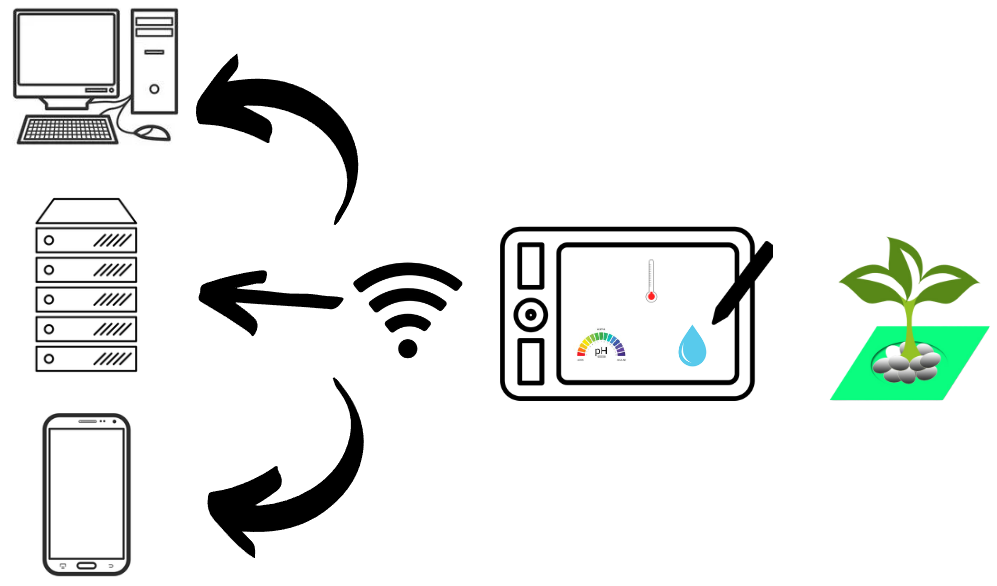
\includegraphics[scale=0.45]{imgs/iot_nueva.PNG} \\
    \caption{Componentes comúnmente utilizados en un sistema de monitoreo basado en IoT. }\label{IoT}
\end{figure}

Algunas de las plataformas, protocolos y tecnologías comúnmente usadas en el desarrollo de sistemas de IoT son:

\begin{itemize}
\item \textbf{Node-Red.} Es un entorno de desarrollo de código abierto (open-source) desarrollado por IBM basado en una programación visual de bloques y nodos que nos ayuda a conectar dispositivos y servicios a través de Internet para realizar tareas específicas, además es una herramienta de desarrollo muy utilizada y de fácil uso junto a las IoT, ya que no requiere conocimientos avanzados de programación y a dado paso a la gestión de datos en tiempo real dando soluciones a la industria 4.0 \cite{NodeRed}.

\item \textbf{MQTT.} Es un protocolo de mensajería (Message Queuing Telemetry Transport), utilizado en aplicaciones de IoT. Este protocolo se basa en ciertas reglas que se definen entre los dispositivos tanto de hardware como software para realizar publicación y suscripciones para compartir datos por Internet. El MQTT se usa comúnmente en el ambiente del Internet industrial para enviar mensajes y obtener parámetros entre los dispositivos, como sensores, controladores lógicos programables, dispositivos integrados, microcontroladores, entre otro más \cite{hillar2018hands}.
 
\item \textbf{Mosquitto.} Es un gestor (\textit{broker}) de mensajes del protocolo de MQTT basado en un modelo Publicación/Subscripción (Pub/Sub). El emisor es el encargado de publicar información de sensores o comandos en un tópico específico y los receptores reciben información a suscribirse al tópico específico, El protocolo MQTT es el intermediario entre los emisores y receptores. El \textit{broker} filtra correctamente todos los mensajes entrantes (publicaciones) y los envía a los suscriptores \cite{ wangconstruction}. 
\end{itemize}

%%%%%%%%%%%REFERENCIA LOGICA DIFUSA%%%%%%%%%%%%%%%%%%%%%

\section{Lógica difusa}
En esta sección se describen los conceptos y el funcionamiento de la lógica difusa. La lógica difusa es un método matemático en el cual se busca imitar el funcionamiento de las expresiones lingüísticas en términos numéricos \cite{zadeh1965fuzzy}. De esa inspiración se parte de la extracción de un modelo de unidades conectadas entre sí, que generan, transmiten y refuerzan conceptos para llegar a conclusiones determinadas y consolidarlas como conocimiento con base en los antecedentes, consecuentes y reglas de inferencia específicas. 

Del modo en el que nosotros expresamos el cómo se encuentra un sistema en términos lingüísticos, la lógica difusa trabaja para tomar dichas expresiones y generar un cambio de una forma más precisa. En el ámbito de la hidroponía, el conocer o predecir valores acerca de los parámetros de un sistema son de suma importancia para asegurar el crecimiento adecuado de las plantas. La lógica difusa permite generar un controlador cuyo funcionamiento está basado en las decisiones que tomaría un experto, para mantener los parámetros en valores requeridos para un sistema hidropónico.

\subsection{Conceptos básicos}
Algunos conceptos usados en control difuso son \cite{passino1998fuzzy}:
\begin{itemize}
\item \textbf{Universo de Discurso.} Rango de todos los valores posibles de la variable del sistema.
\item \textbf{Rango o Dominio.} Intervalo sobre la cual una función de membresía es mapeada.
\item \textbf{Término lingüístico.} Es un conjunto de variables, con un lenguaje natural que puede expresar los posibles valores de las variables. Tome $"Altura"$ como ejemplo, que tiene los siguientes tipos: bajo, medio, alto. Estos se denominan términos lingüísticos y representan los posibles valores de los términos. Entonces la variable puede ser más o menos relacionado con los términos lingüísticos. El conjunto de términos lingüísticas es un conjunto difuso cuando su grado de certeza sea un valor de un término en sí, dado a sus condiciones según sus respectivas funciones de membresía.
\item \textbf{Función de membresía.} Es la curva que define la forma de cada punto en el espacio. La entrada toma un valor de pertenencia entre 0 y 1. El espacio de entrada se denomina universo del discurso. Algunas de las formas de funciones de membresía se presentan en la figura \ref{funcion}. 
\begin{figure}[!ht]
\centering
         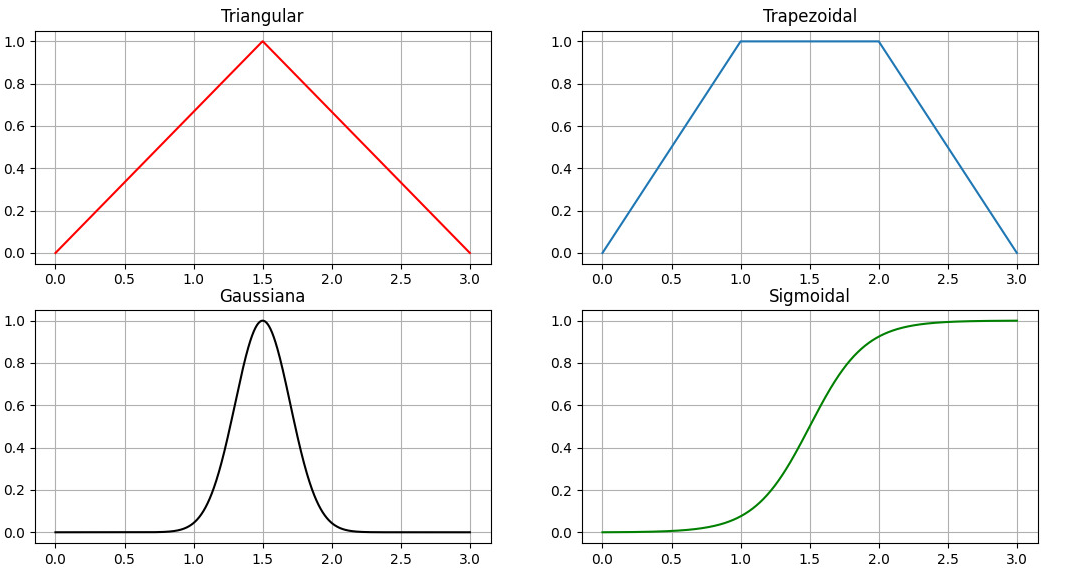
\includegraphics[scale=0.55]{imgs/funciones.png} \\
    \caption{Tipo de funciones de membresía.} \label{funcion}
\end{figure}

\item \textbf{Reglas SI-ENTONCES}:Las reglas de inferencia son conclusiones condicionales que controlan el sistema. Cada regla se compone de un antecedente y un consecuente.
\begin{center}
SI x es A ENTONCES y es B
\end{center}

Donde A y B son valores lingüísticos definidos por conjuntos difusos en los rangos X e Y, respectivamente. La parte de la regla "x es A" se llama el antecedente o premisa, mientras que la parte de la regla " y es B" se llama consecuente. 
\end{itemize}
\section{Control Automático}
El control automático es una disciplina de la ingeniería que se ocupa del diseño e implementación de sistemas que permitan automatizar procesos y aumentar su eficiencia y calidad. Los sistemas de control automático se utilizan en una variedad de aplicaciones, desde el control de temperatura y presión en procesos industriales hasta el control de velocidad y dirección en vehículos autónomos. El control automático se basa en la retroalimentación, es decir, en la base de la medición del estado del sistema y la comparación de este estado con un punto de ajuste de referencia. Con base en esta comparación, el sistema de control ajusta los parámetros del proceso para mantener el sistema en el estado deseado. Los sistemas de control automático se pueden dividir en diferentes categorías según su complejidad y aplicación \cite{ogata2010modern}. Las principales categorías son:
\begin{itemize}
    \item \textbf{Controlador Proporcional Integral Derivativo (PID).} Este es el sistema de control más común y tiene una amplia gama de aplicaciones. El controlador PID ajusta el parámetro del proceso en función del error entre el punto de referencia y la medición real, el error integral y el error derivado.
    \item \textbf{Controlador lógico programable (PLC, por sus siglas en inglés).} Es un sistema de control programable utilizado para automatizar procesos y equipos industriales. Los PLC están programados para tomar decisiones en función de las entradas de los sensores y la lógica de control predefinida.
    \item \textbf{Controlador difuso.} Son sistemas de control basados en la lógica difusa y se utilizan en aplicaciones en las que el sistema no se puede describir con precisión mediante ecuaciones matemáticas \cite{mamdani1975experiment}.
    \item \textbf{Controlador por medio redes neuronales.} son sistemas de control basados en la simulación de redes neuronales artificiales y se utilizan en aplicaciones donde el sistema es muy complejo o no se puede modelar con precisión \cite{bishop1995neural}.
\end{itemize}

\subsection{Control difuso}
Es un sistema de control que utiliza lógica difusa para controlar un proceso o sistema. En un controlador difuso, la entrada y la salida del sistema se describen mediante conjuntos que representan la incertidumbre y la inexactitud de las medidas y el conocimiento del sistema \cite{mamdani1975experiment}  \cite{ross2009fuzzy}.
\\
El modelo de un controlador difuso se divide en 4 etapas, estas se pueden observar en la figura \ref{difuso}:
\begin{figure}[!ht]
\centering
         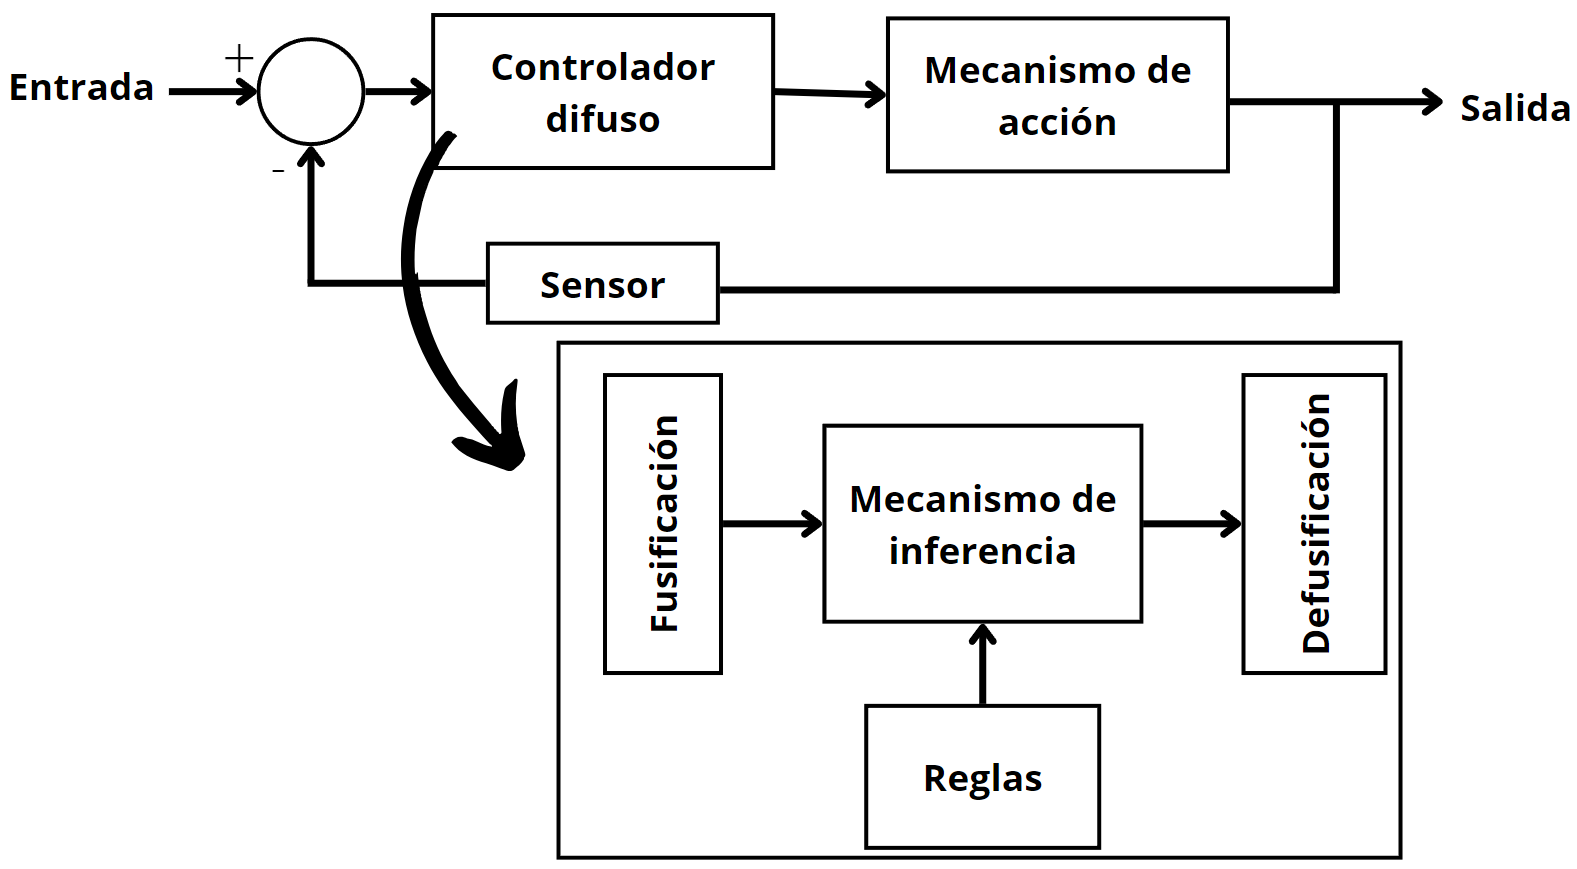
\includegraphics[scale=0.36]{imgs/Diagramacontrol.png} \\
    \caption{Modelo de un controlador difuso.}\label{difuso}
\end{figure}
\begin{itemize}
    \item \textbf{Parámetros previos.} Para crear un controlador difuso, primero se deben definir las variables de entrada y salida del sistema. Estas variables pueden ser físicas, como la temperatura o la presión, o abstractas, como la satisfacción del cliente en un restaurante. Las variables de entrada y salida se describen mediante conjuntos difusos definidos por funciones de membresía, tal y como se mencionó en la \textit{Sección 2.3 Lógica difusa.}

    \item \textbf{Fusificación.} Es el proceso en el que se transforman las entradas en términos lingüísticos que puedan ser procesados por el controlador. La fusificación es necesaria debido a que las variables pueden contener incertidumbre, imprecisión o ambigüedad. La fusificación se realiza en dos etapas principales: la asignación de los valores de entrada a los conjuntos difusos y la determinación de los grados de pertenencia de los valores de entrada y salida en cada conjunto.
    \item \textbf{Mecanismo de inferencia y reglas de inferencia.} Una vez definidas las variables de entrada y salida, se deben crear las reglas del sistema difuso. Estas reglas describen la relación entre las variables de entrada y salida del sistema. Por ejemplo, La velocidad de un ventilador en cierta área de trabajo, si la temperatura del área es alta y la presión es baja. Las reglas son basadas en la lógica difusa mediante operadores de unión, intersección y negación, y se pueden combinar para formar reglas complejas.

    \item \textbf{Defusificación.} En la última etapa en el proceso de un control difuso, se convierte la salida difusa del controlador en una salida precisa y útil para el sistema de control. La defusificación se realiza para convertir los valores lingüísticos de la salida del controlador difuso en un valor numérico que pueda ser utilizado para controlar el sistema, dentro de este proceso existen diferentes metodologías como bisectriz, primer máximo, último máximo, media de máximos, centroide, entre otros más.



\end{itemize}






\section{Visión por computadora}
La visión por computadora es un campo de la inteligencia artificial que se enfoca en desarrollar algoritmos y sistemas que pueden procesar y analizar imágenes y videos para extraer información y conocimiento de ellos. La visión por computadora es un campo muy importante en la robótica, la seguridad, la medicina, la publicidad, la industria del entretenimiento y muchos otros. Esta se basa en la capacidad de los algoritmos para procesar imágenes digitales y reconocer patrones en ellas. Para ello se utilizan técnicas de procesamiento de imágenes como el filtrado, la segmentación, la extracción de características, el reconocimiento de objetos y la detección de movimiento.

Las aplicaciones incluyen la clasificación de imágenes, la detección de objetos, el seguimiento de objetos en movimiento, el reconocimiento facial, el reconocimiento de objetos en imágenes médicas, la detección de defectos en la fabricación industrial y el reconocimiento de objetos en imágenes satelitales \cite{szeliski2010computer}.
En pocas palabras, la visión por computadora es una disciplina interdisciplinaria que utiliza la tecnología en constante evolución que contienen un enorme potencial para crear información mediante imágenes y videos.

\subsection{Segmentación de imágenes}
La segmentación es un paso importante en el procesamiento de imágenes que se refiere al proceso de dividir una imagen en regiones o segmentos significativos. La segmentación es una tarea clave en la visión por computadora para el uso de reconocimiento de objetos y la detección de bordes. Existen varias técnicas para la segmentación de imágenes utilizando la visión por computadora:
\begin{itemize}
    \item \textbf{Umbral:} Es un método de segmentación simple en el que se elige un umbral y cada píxel de la imagen se clasifica en función de su valor está por encima o por debajo del umbral. Esta técnica se utiliza cuando se desea distinguir claramente el fondo de una imagen o video. 
    \item \textbf{Segmentación basada en bordes:} Este método se basa en la detección de bordes en una imagen, lo que ocurre cuando hay cambios significativos en la intensidad de la imagen.
    \item \textbf{Segmentación por regiones}: este método de segmentación se basa en agrupar píxeles en regiones con propiedades similares, como el color, la textura o la intensidad. 
    \item \textbf{Segmentación semántica:} la segmentación semántica utiliza técnicas de aprendizaje profundo para segmentar una imagen en regiones que corresponden a objetos y características específicas de la imagen. Este método es útil para aplicaciones que requieren reconocimiento de objetos de alta precisión. 
\end{itemize}
La elección de una técnica de segmentación adecuada depende del tipo de imagen, la calidad de la imagen y la tarea específica a realizar.
    